\chapter*{Week 2: Conditionals}
\addcontentsline{toc}{chapter}{Week 2: Conditionals}
\setcounter{chapter}{2}
\setcounter{section}{0}

\begin{abstract}
This week will cover:
\begin{enumerate}
    \item Characters 
    \item Switch Statements
    \item Learn about a new variable type: Booleans
    \item Learn about Boolean Logic and be able to fill in truth tables
    \item Learn about conditional statements:
    \begin{itemize}
        \item If statements
        \item If/Else Statements
        \item If/Elif/Else Statements
        \item Nested If/Else Statements
    \end{itemize}
\end{enumerate}
    
\end{abstract}

\section{Background}

\subsection{Characters}

Characters are a variable type that is made of a single byte, which means they can encode for a fairly limited number of characters. We can identify which characters we can store using an ASCII table shown below. 

Characters can be referred to by placing the chosen character in single quotation marks, like this:

\mintinline{c++}{char myChar = 'a';}

Characters can also can be accessed using numerical values. Since every sequence of binary numbers that encodes a character could also instead be interpreted as an integer, we can use those numbers to identify which character we are talking about. The integer values that correspond with each letter are shown in the ASCII table.

There are a few traits that you may find helpful as you move forward: firstly, observe that all lower case letters are listed in consecutive alphabetical order, and secondly that all upper case letters are similarly listed in consecutive alphabetical order. This means that the space between a lowercase `a' and a capital `A' is the same as the space between a lowercase `b' and a capital `B' and so on. This is useful for converting characters from lowercase to uppercase. 

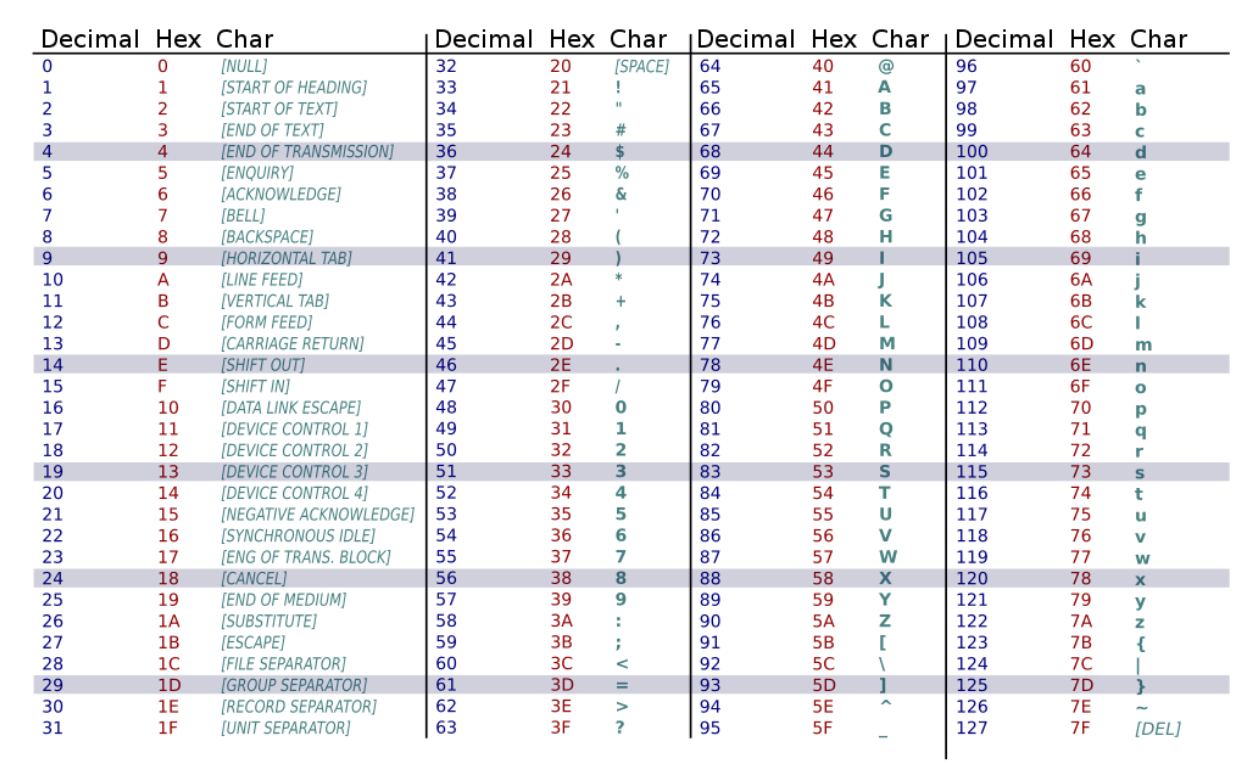
\includegraphics[width=\textwidth]{images/ascii_table.png}

\subsection{Switch Statements}

We have discussed variables, and a couple ways to manipulate variables so far. But what happens if you don't always want to do the same thing? 

Switch statements are an easy way to make decisions in code. Based on the value of a character or integer variable we can execute different sections of code. 
\begin{itemize}
    \item If we are building a switch statement around an \mintinline{c++}{int} variable, all of the cases must be defined using numbers. 
    \item If we are building a switch statement around a \mintinline{c++}{char} variable, all of the cases must be defined using characters. This means they must also use single quotes. 
\end{itemize}

\begin{center}
    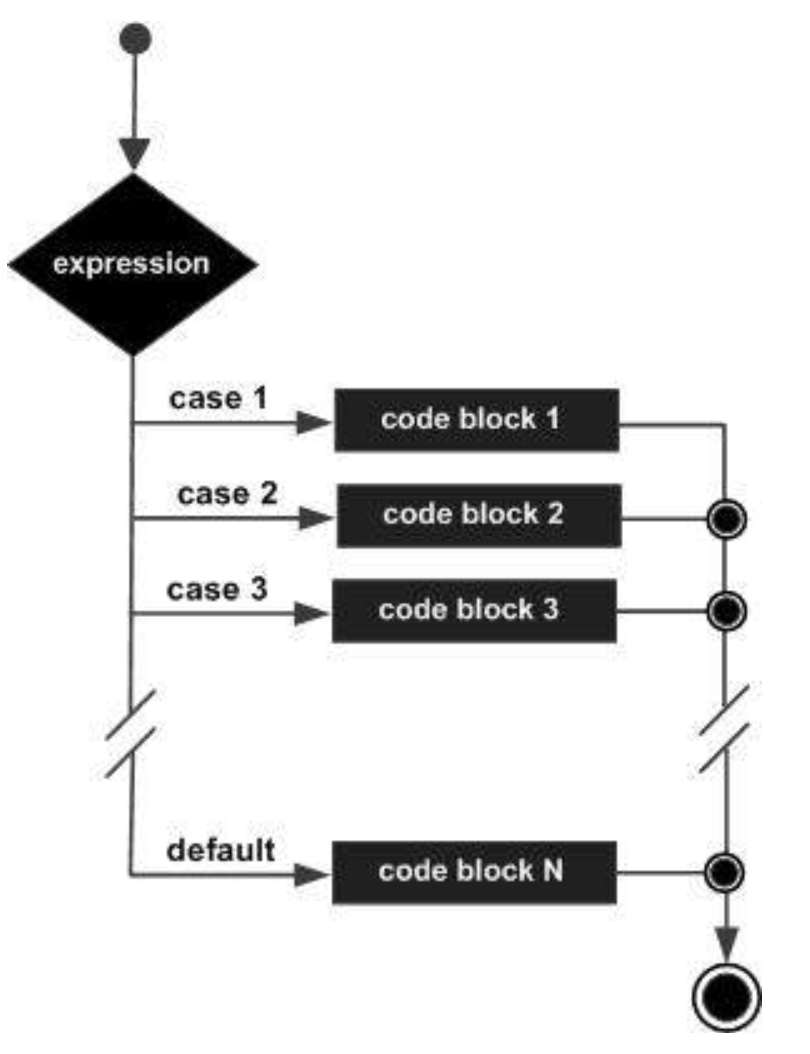
\includegraphics[width = \textwidth /2]{images/switchdiagram.png}
\end{center}

With the switch statement, the variable name is used once in the opening line. A case keyword is used to provide the possible values of the variable, which is followed by a colon and a set of statements to run if the variable is equal to a corresponding value.

An example of a simple switch statement:

\begin{example}
    Switch statement syntax:
\begin{minted}{c++}
switch (n){
     case 1:
          // code to be executed if n == 1;
          break;
     case 2:
          // code to be executed if n == 2;
          break;
     default:
          // code to be executed if n doesn’t match any cases
}
\end{minted}
\end{example}

Important notes to keep in mind when using switch statements :

\begin{itemize}
    \item The expression provided in the switch should result in a constant value otherwise it would not be valid.
    \begin{itemize}
        \item \mintinline{c++}{switch(num)}
        \begin{itemize}
            \item allowed (\mintinline{c++}{num} is an integer variable)
        \end{itemize}
        \item \mintinline{c++}{switch('a')}
        \begin{itemize}
            \item allowed (takes the ASCII Value)
        \end{itemize}
        \item \mintinline{c++}{switch(a+b)}
        \begin{itemize}
            \item allowed, where \mintinline{c++}{a} and \mintinline{c++}{b} are \mintinline{c++}{int} variables, which are defined earlier
        \end{itemize}
    \end{itemize}
    \item The \mintinline{c++}{break} statement is used inside the switch to terminate a statement sequence. When a \mintinline{c++}{break} statement is reached, the switch terminates, and the flow of control jumps to the next line following the switch statement.
    \item The \mintinline{c++}{break} statement is optional. If omitted, execution will continue on into the next case. The flow of control will fall through to subsequent cases until a break is reached.
    \item The default statement is optional. Even if the switch case statement does not have a default statement, it would run without any problem.
\end{itemize}

Switch statements are a simple way to make decisions based exclusively on the equivalence of some characters or numbers. They are a simple form of \textbf{conditional statement}, and we will examine a few more complicated versions next week. 

\subsection{Booleans}
Booleans are a special data type that stores only ``true" or ``false". This true or false value can be stored in a boolean variable, or it can be the result of evaluating different expressions.

\subsubsection{Relational Operators}
A relational operator is a feature of a programming language that tests or defines some kind of relation between two entities. These include numerical equality (e.g., \mintinline{c++}{5 == 5}) and inequalities (e.g., $4 \geq 3$). Relational operators will evaluate to either True or False based on whether the relation between the two operands holds or not. When two variables or values are compared using a relational operator, the resulting expression is an example of a boolean condition that can be used to create branches in the execution of the program. Below is a table with each relational operator’s C++ symbol, definition, and an example of its execution.

\begin{table}[H]
    \centering
    \begin{tabular}{c|c|c}
        Operator & Meaning & Example \\ \hline
        $>$ & greater than & $5 > 4$ is TRUE \\
        $<$ & less than & $4 < 5$ is TRUE \\
        $>=$ & greater than or equal & $4 >= 4$ is TRUE \\
        $<=$ & less than or equal & $3 <= 4$ is TRUE \\
        == & equal to & $5 == 5$ is TRUE \\
        != & not equal to & $5 != 6$ is TRUE
    \end{tabular}
\end{table}

\subsubsection{Logical Operators}
Logical operators are used to compare the results of two or more conditional statements, allowing you to combine relational operators to create more complex comparisons. Similar to relational operators, logical operators will evaluate to True or False based on whether the given rule holds for the operands. Below are some examples of logical operators and their definitions.

\begin{table}[H]
    \centering
    \begin{tabular}{c|c|c}
    \mintinline{c++}{&&} & AND & returns true if and only if both operands are true\\
    \mintinline{c++}{||} & OR & returns true if one or both operands are true \\
    ! & NOT & returns true if the operand is false and false if the operand is true
    \end{tabular}
\end{table}

Every logical operator will have a corresponding truth table, which specifies the output that will be produced by that operator on any given set of valid inputs. Below are truth tables for each of the logical operators specified above.

AND ( \mintinline{c++}{&&} ): These operators return true if and only if both operands are True. This can be visualized as a venn diagram where the circles are overlapping.

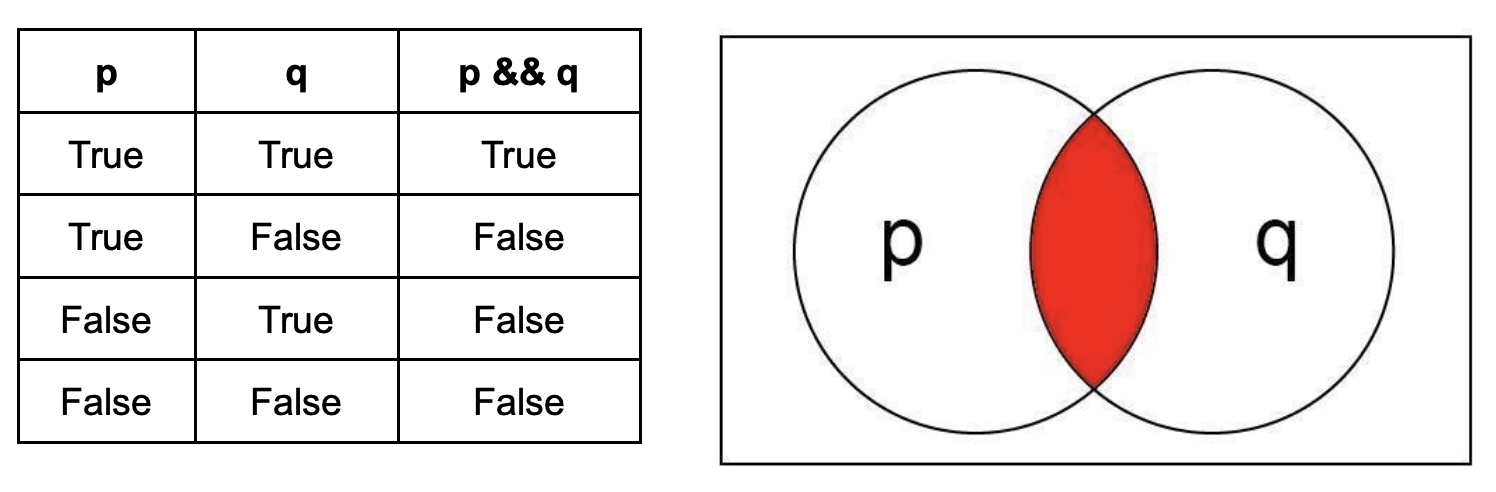
\includegraphics[width=\textwidth]{images/and.png}

OR ( \mintinline{c++}{||} ): These operators return True if one or both of the operands are True. This can be visualized as the region of a venn diagram encapsulated by both circles.

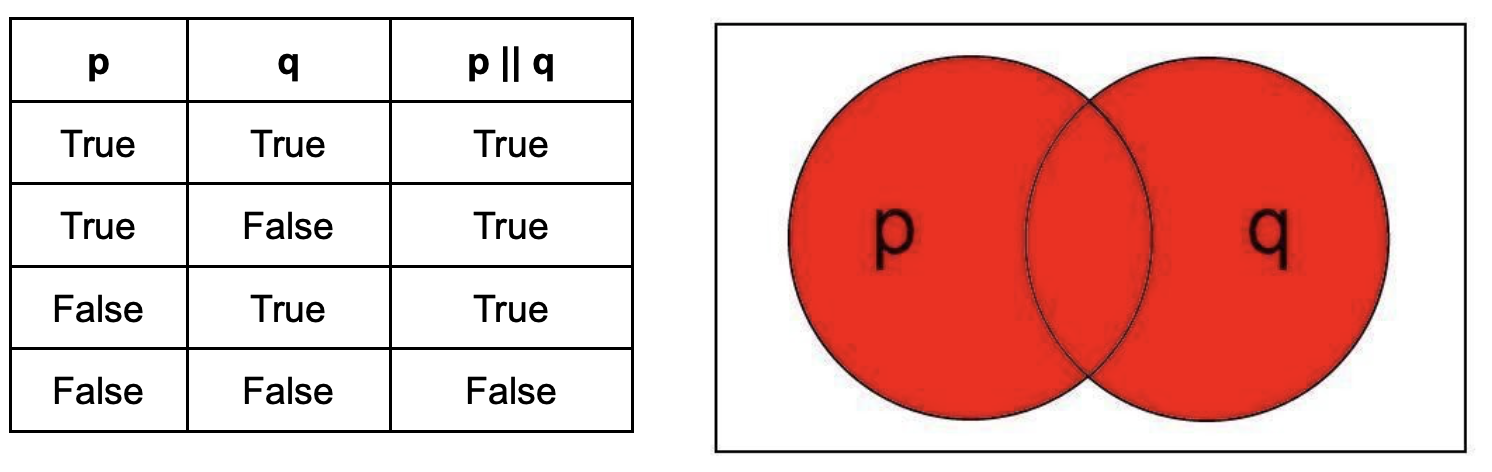
\includegraphics[width=\textwidth]{images/or.png}

NOT ( ! ): This operator returns the opposite of the operand. This can be visualized as the region of a venn diagram outside the circle. Unlike AND and OR, the NOT operator has only one operand.

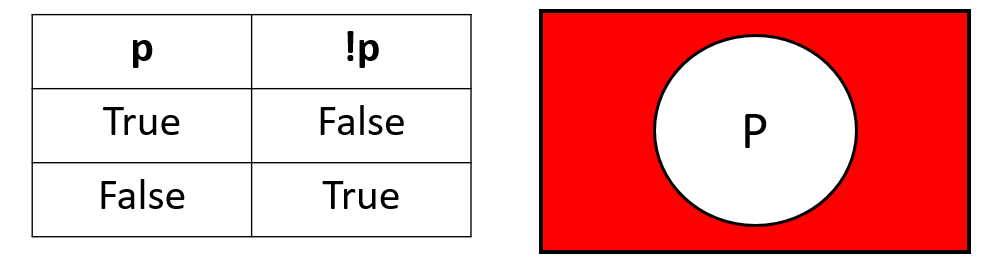
\includegraphics[width=\textwidth]{images/not.png}

You can create truth tables for more complicated expressions by combining elements of these tables. You should begin with columns of the basic variables representing each possible combination of those variables, and then add columns to represent their modified values. For example, if you wanted to create a truth table for \mintinline{c++}{!p && q} you could make a column for \mintinline{c++}{p} and a column for \mintinline{c++}{q} representing all possible combinations of true/false between the two variables. You can then create a third column for \mintinline{c++}{!p}, and then perform the \mintinline{c++}{&&} operation between the \mintinline{c++}{!p} and \mintinline{c++}{q} columns instead of the \mintinline{c++}{p} and \mintinline{c++}{q} columns, like this below:

\begin{table}[H]
    \centering
    \begin{tabular}{c|c|c|c}
        \mintinline{c++}{p} & \mintinline{c++}{q} & \mintinline{c++}{!p} & \mintinline{c++}{!p && q} \\ \hline
        True & True & False & False \\
        True & False & False & False \\
        False & True & True & True \\
        False & False & True & False
    \end{tabular}
\end{table}

For simple expressions, you can often work through the truth table in your head. However, knowing how to make truth tables will be helpful when you need more complicated expressions.

\subsubsection{Using Booleans}
There are two main ways you can use booleans: you can either assign them to a boolean variable, or you can use them directly as a condition (such as in an if statement). If you would like to evaluate a boolean expression and store it in a variable, you can do it like this:

\begin{minted}{c++}
    bool myNewBoolean = (4 < 5); // this will evaluate to true
    bool mySecondBoolean = (5 == 6); //this will evaluate to false
    bool myFinalBoolean = (myNewBoolean && mySecondBoolean); //this will evaluate to false
\end{minted}

You can string together increasingly complicated boolean equations either as a combination of boolean variables or as a combination of relational/logical expressions.

Booleans can also be represented using integers, and will print that way by default in C++. As an integer representation, 0 is false and 1 is true. 

You can build if statements using boolean variables or boolean expressions.

\subsection{Conditionals}
Conditional statements, also known as decision statements or branching statements, are used to make a decision based on condition. A condition is an expression that evaluates to a boolean value, either true or false. \href{https://cal-linux.com/tutorials/conditionals.html}{\textcolor{cyan}{Conditional Execution in C++}} is a good online resource for learning about conditionals in C++.

You have seen one type of conditional expression already: switch statements. If statements, If/Else statements, and If/Else If/Else statements are a more complicated but also more dynamic way to make decisions in your code.

\subsubsection{IF Statements} 

An if statement in C++ is composed of a condition and a body. The body is executed only if the condition is true. The condition appears inside a set of parentheses following the keyword “if” and the body appears within a set of curly brackets after the condition:

The general format for if statements is:

\begin{minted}{c++}
if ( <CONDITION> ){
	<BODY>
}    
\end{minted}

It is good practice to vertically align the closing curly bracket with the start of the if statement, and to indent the body.

The condition is interpreted as a boolean value, either true or false. Be careful, most expressions in C++ have a boolean interpretation. For instance, non-zero numeric values are true. Assignment operations (single equal sign) are interpreted as true as well. A common mistake is to use a single equals sign inside a condition when a double equals sign is intended.

\begin{example}
    Here is an if statement that will check if a number is negative and change it to positive (i.e., find the absolute value):

    \begin{minted}{c++}
if (num < 0){
	cout << "Changing sign" << endl;
	num = -1 * num;
}
    \end{minted}
\end{example}

\subsubsection{IF-ELSE Statements}
 If statements may be paired with else statements in C++. If the condition associated with the if statement is false, the body associated with the else statement is executed. The else statement body is enclosed in a set of curly brackets:

 \begin{minted}{c++}
 if ( <CONDITION> ){
	<BODY>
    // executed when CONDITION is true
}
else{
	<BODY>
    // executed when CONDITION is false
}
 \end{minted}

 An if statement does not need an else statement, but there must be an if statement before every else statement.

 \begin{example}
     Here is an if/else statement that will check if a number can be a divisor before performing division:
     \begin{minted}{c++}
if (num == 0) //notice the double equals!{
	cout << "Can't divide by 0!" << endl;
}
else{
	num = 1000 / num; //integer arithmetic
}         
     \end{minted}
 \end{example}

 \subsection{ELSE-IF Statements}
 
 Finally, an if statement may also be associated with any number of else-if statements. These statements each have an associated condition and an associated body. The body is executed if the condition is true and the conditions for all preceding if- and else-if statements in the same group are false. An else statement may be included at the end of the group but is not required. The else statement will be executed if all the previous conditions are false.

\begin{minted}{c++}
if ( <CONDITION> ){
	<BODY>
}
else if ( <CONDITION> ){
	<BODY>
}
else if ( <CONDITION> ){
	<BODY>
}
else{
	<BODY>
}
 \end{minted}

 This is \textbf{not} logically the same as having multiple sequential if statements. 

 \begin{example}
     These two if statements:
     \begin{minted}{c++}
         if ( <CONDITION A>){
            //do X
         }
         if ( <CONDITION B>){
            //do Y
         }
     \end{minted}
     are NOT logically the same as this if/else-if statement:
     \begin{minted}{c++}
         if( <CONDITION A>){
            //do X
         }
         else if ( <CONDITION B>){
            //do Y
         }
     \end{minted}
 \end{example}

 In the first code section, both if statements are evaluated. If both CONDITION A and CONDITION B are true, we will do \textbf{both} X and Y. Meanwhile, in the second code block, if CONDITION A is true we will never evaluate CONDITION B, and therefore never do execute that code; here, we will \textbf{only} do X. Therefore, we need to use ``else if" only when we want the two conditions to be mutually exclusive.

 \begin{example}
     Here is an if/else if/else statement to tell you if a number is positive, 0, or negative:
\begin{minted}{c++}
if ( num > 0 ){
	cout << "Positive" << endl;
}
else if ( num == 0 ){
	cout << "Zero" << endl;
}
else{
	cout << "Negative" << endl;
}
\end{minted}
 \end{example}

 \subsubsection{Nested If Statements}
 You can put if statements inside of other if statements (or if/else, or if/else if/else). The meaning of logical expressions can change when you are nesting if statements, so you should think through the truth tables for your if/else statements carefully. 

 \begin{minted}{c++}
     if (booleanExpression1){
        //anything here will evaluate if booleanExpression1 is true
        if (booleanExpression2){
            //we will only evaluate this if statement if booleanExpression1 is true, 
            //and then will only execute this statement if booleanExpression2 is ALSO true
        }
     }
 \end{minted}

 Nested if statements are essentially performing a logical ``AND" operation on the two boolean expressions for the innermost if statement, but if only the first if statement is true you can still do other things. 

\subsection{Common Errors}
Unintended behavior when accidentally using assignment operation (= instead of ==) in conditional statements:

\begin{example}
    Here is some (incorrect) code:

    \begin{minted}{c++}
    int x = 5;
    if (x = 1){ // one equal sign: changes value of x, will always evaluate to true
    
    	cout << "The condition is true." << endl;
    }
    cout << "x is equal to " << x << endl;
    \end{minted}
    The output of this would look like this:
    \begin{sample}
The condition is true.

x is equal to 1
    \end{sample}
    What you would ACTUALLY want is:
    \begin{minted}{c++}
    // CORRECT CODE
    int x = 5;
    if (x == 1) // two equal signs, performs comparison
    {
    	cout << "The condition is true." << endl;
    }
    cout << "x is equal to " << x << endl;
    \end{minted}
    Which would output:
    \begin{sample}
x is equal to 5
    \end{sample}
\end{example}

Remember, ``=" is for assignment and ``==" is for checking equality.



\section{Warmup}

\begin{problem}
    Fill in the blank(s) for the code below:
    \begin{minted}{c++}
    char choice;
    cout << "Play rock paper scissors! Enter R, P, or S." << endl;
    ______ >> choice;

    switch(________){
        case _______:
            cout << "You chose rock. I also chose rock, so we tie." << endl;
            break;
        case 'P':
            cout << "You chose paper. I chose rock, so you win." << endl;
            _________
        case 'S':
            cout << ____________________________ << endl;
            break;
        default:
            cout << "That's not a valid choice! Cheater." << endl;
    }
    \end{minted}
\end{problem}

\begin{problem}
Below is code that asks the user for the day of the week as a number (Monday is 1, Sunday is 7) and then prints a corresponding statement. Identify the error(s):
\begin{minted}{c++}
    int day;
    cout << "What number day of the week is it?" << endl;
    cin >> day;
    switch (day) {
      case '6':
        cout << "Today is Saturday";
        break;
      case 7:
        cout << "Today is Sunday";
        
      default:
        cout << "Looking forward to the Weekend";
    }
\end{minted}

\end{problem}

\begin{problem}
    Below is code with the same goal as the previous question, but different error(s). Identify the error(s):
    \begin{minted}{c++}
    int day = 4;
    switch (day) 
      case 6:
        cout << "Today is Saturday";
        break;
      case 7:
        cout << "Today is Sunday";
        break;
      default
        cout << "Looking forward to the Weekend";
        
    \end{minted}
\end{problem}

\begin{problem}
    Spot the error(s):
    \begin{minted}{c++}
    #include <iostream>
    using namespace std;
    
    int main()
    {
        int angle =40;
        if (x<90) { 
            cout<<"It is an acute angle." ;
        }
        else if(x=90) {
            cout<<"It is a right angle.";
        }
        els{
            cout<<"It is an obtuse angle.";
        }
    }
    \end{minted}
\end{problem}

\begin{problem}
    Spot the error:
    \begin{minted}{c++}
    // This program implements XOR
    #include iostream
    using namespace std;
    
    //Set the variable value to 1 when x or y is 1
    int main(){				
        int x = 1,y=0,value;
        
        if (x == 1){ 
            if(y==0)
            value = 1; 
    
            else
            y == 0; 
         
        if(x==0){ 
            if(y==0)
            value = 0; 
    
            else
            value = 1;
        }
        
        cout < value < endl;
        return 0;
    }
    \end{minted}
\end{problem}


\section{Recitation}
\subsection{Step Tracking App}
Your goal is to walk 10,000 steps every day but you aren’t great at remembering to do it! So you decide to create a step tracking app that tracks your steps every day and will alert you based on how much you walked for the day. The program first asks how many steps you walked that day and then displays a message based on whether you have hit your goal for the day. Next, it will also tell you how many steps you have left to walk.

The following are the possible messages you will get based on your intake:

\begin{itemize}
    \item If you've walked 5,000 steps or less, then you get: 
    
    \mintinline{text}{You have not walked much today! Get those steps in! You have X steps left to walk.}
    
    \item If you’ve walked more than 5,000 steps but less than 10,000 steps, you get: 
    
    \mintinline{text}{You're doing great, over half way there! You still have X steps left to walk.}

    \item If you've walked 10,000 steps or more, you get:
    
    \mintinline{text}{You've hit your goal for the day! Great job getting exercise!}
\end{itemize}

Note that \textbf{X} is the amount of steps left after subtracting how far you have walked. 

Here is a sample run:

\begin{sample}
How many steps have you taken today?

\textcolor{red}{3000}

You have not walked much today! Get those steps in! You have 7000 steps left to walk.
\end{sample}

\begin{multipart}
    Write an algorithm in pseudocode for the program above.
\end{multipart}

\vspace{4cm}

\begin{multipart}
     Imagine how a sample run of your program would look like. Write at least two examples.
\end{multipart}

\vspace{4cm}

\begin{multipart}
    Identify the values that you must test for. We call these values ``boundary conditions".
\end{multipart}

\vspace{4cm}

\begin{multipart}
    Implement your solution in C++ using VS Code. Revise your solution, save, compile and run it again. Are you getting the expected result and output? Keep revising until you do. Make you sure you test for the values used in your sample runs, and for the boundary conditions. 
\end{multipart}

\subsection{Grade Calculator}
You want to create a grade calculator. You will need two conditions: one to determine the letter grade, and one to determine the symbol with the letter (+, -, or empty). 

\begin{multipart}
    How can you take a numerical grade (on a scale of 0-100) and convert it to a letter grade?
\end{multipart}

\vspace{4cm}

\begin{multipart}
    How can you take a numerical grade (on a scale of 0-100) and find the appropriate symbol? Are there any special values you should consider? Do all grade ranges get associated with a symbol?
\end{multipart}

\vspace{4cm}

\begin{multipart}
    Write your two conditions and test them by asking the user for their grade as a percentage, and then printing the result of both your functions. Make sure to test a variety of values.
\end{multipart}

\section{Homework}
\subsection{Tubing in Boulder Creek}
Write a C++ program that will determine if it is safe to go tubing in Boulder Creek. The maximum flowrate to go tubing is 250 cfs (cubic feet per second).

The program should take an integer input from the user and display one of the two phrases to the user (unless input is invalid).

\begin{sample}
What is the flowrate of Boulder Creek?

\textcolor{red}{109}

It is safe to go tubing. Have fun!
\end{sample}

\begin{sample}
What is the flowrate of Boulder Creek?

\textcolor{red}{461}

The river is flowing too fast to go tubing.
\end{sample}

\begin{sample}
What is the flowrate of Boulder Creek?

\textcolor{red}{-453}

Please enter a valid input.
\end{sample}

Make sure your program does basic input validation. The flowrate must be greater than zero. If the user inputs a non-positive value, print Please enter a valid input. and exit the program.

\subsection{Ordering Pizza}
You've decided to order a pizza for dinner. The restaurant you're ordering from has three sizes of pizza: S, M, and L. Each size has a different base price and price per topping. The prices are indicated in the table below. Create a program to calculate the total cost of your pizza. The program should prompt you for the size of pizza and the number of toppings, then output the cost.

\begin{table}[H]
    \centering
    \begin{tabular}{c|c|c}
        Size & Base Price & Price Per Topping \\
        S & 8.00 & 0.99 \\
        M & 10.00 & 1.99 \\
        L & 14.00 & 2.99
    \end{tabular}
\end{table}

The input should be a character (for size) and non-negative integer (for number of toppings) and the output should be a double. 

Note: The total cost should be formatted with a two-digit precision. You can use the \mintinline{c++}{setprecision()} function with the fixed manipulator from \mintinline{c++}{<iomanip>} library to do so.

Bad formatting: 10.8

Good formatting: \$10.80

You will also need to perform input validation on the size of the pizza -- i.e., XL is not valid. 

\begin{sample}
What size pizza would you like to order?

\textcolor{red}{S}

How many toppings do you want?

\textcolor{red}{3}

Your total is \$10.97
\end{sample}

\begin{sample}
What size pizza would you like to order?

\textcolor{red}{M}

How many toppings do you want?

\textcolor{red}{1}

Your total is \$11.99
\end{sample}

\subsection{Wifi Speeds}

You've decided to test the temperature outside every morning. Create a program that will tell you if the temperature over the last three days has increased, decreased, or neither. If the temperatures are sorted and increasing, then print out "It's getting warmer!". If the temperatures are sorted and decreasing, then print out "It's getting cooler!". If the temperatures are unsorted or if two or more temperatures are the same, then print "The temperature is changing unpredictably."

The user should input 3 non-negative numbers (double) separated by spaces.

\begin{sample}
Enter temperatures over the last three days:

\textcolor{red}{75 79 81}

It's getting warmer!
\end{sample}

\begin{sample}
Enter temperatures over the last three days:

\textcolor{red}{45 30 18}

It's getting cooler!
\end{sample}

\begin{sample}
Enter temperatures over the last three days:

\textcolor{red}{79 75 90}

The temperature is changing unpredictably.
\end{sample}

\subsection{Class Enrollment}
You want to create a program to enroll in classes. You've narrowed the class list down to just a few classes that computer science students might need.

In your program, first the user will select a department and the program will tell them what classes are available from that department. Then the user picks a class and you will print a confirmation message that they have enrolled in the class. The classes are as follows:

\begin{table}[H]
    \centering
    \begin{tabular}{c|c}
        Math &  Linear Algebra\\
        & Multivariate Calculus\\
        & Abstract Math \\ \hline
        Computer Science & Starting Computing \\
        & Data Structures \\
        & Discrete Structures \\ \hline
        Science & General Chemistry 1 \\
         & Physics 1
    \end{tabular}
\end{table}

You will need to do input validation for all stages -- for the department as well as for the course. Sample input/output are shown below:

\begin{sample}
    Would you like to register for a math(m) class, a computer science(c) class, or a science(s) class?

    \textcolor{red}{m}

    Would you like to register for Linear Algebra (1), Multivariate Calculus (2), or Abstract Math (3)?

    \textcolor{red}{2}

    You have been registered for Multivariate Calculus. 
\end{sample}

\begin{sample}
    Would you like to register for a math(m) class, a computer science(c) class, or a science(s) class?

    \textcolor{red}{Q}

    That is not a valid selection.
\end{sample}

\begin{sample}
    Would you like to register for a math(m) class, a computer science(c) class, or a science(s) class?

    \textcolor{red}{s}

    Would you like to register for General Chemistry 1 (1) or Physics 1 (2)?

    \textcolor{red}{3}

    That is not a valid selection.
\end{sample}

